\documentclass[solutionorbox,answers]{exam}


%%%%%%%%%%%%%%%%%%%%%%%%%%%%%%%%%%%%%%%%%%%%%%%%%%%%%%%%%%%%%%%
% Update to change header
\newcommand{\courseName}{CS 577}
\newcommand{\assignmentName}{Assignment 8 -- More Dynamic Programming}
\newcommand{\semester}{Fall 2023}
%%%%%%%%%%%%%%%%%%%%%%%%%%%%%%%%%%%%%%%%%%%%%%%%%%%%%%%%%%%%%%%

\usepackage[utf8]{inputenc}
\usepackage[T1]{fontenc}

\usepackage{amsmath}
\usepackage{amsfonts}
\usepackage{amsthm}
\usepackage{booktabs}
\usepackage{listings}
\usepackage[ruled]{algorithm2e}
\usepackage{graphicx}
\usepackage[rightcaption]{sidecap} 

\usepackage{listings}
\lstset{basicstyle=\ttfamily,
  showstringspaces=false,
  commentstyle=\color{red},
  keywordstyle=\color{blue}
}

\usepackage{hyperref}

\pagestyle{headandfoot}
\runningheadrule
\firstpageheader{\courseName}{\huge \assignmentName}{\semester}
\runningheader{\courseName}
{\assignmentName}
{\semester}
\firstpagefooter{}{}{}
\runningfooter{}{Page \thepage\ of \numpages}{}

\begin{document}

\begin{center}
\fbox{\parbox{5.5in}{\centering
Answer the questions in the boxes provided on the
question sheets. If you run out of room for an answer,
add a page to the end of the document. \\
\vspace{0.1in}
}}
\end{center}
\vspace{0.1in}
\makebox[0.48\textwidth]{Name:\enspace Riya Kore \hrulefill} \qquad
\makebox[0.48\textwidth]{Wisc id:\enspace rykore \hrulefill}

\section*{More Dynamic Programming}

Do \textbf{NOT} write pseudocode when describing your dynamic programs. Rather give the Bellman Equation, describe the matrix, its axis and how to derive the desired solution from it.
\begin{questions}
\question \textit{Kleinberg, Jon. Algorithm Design (p. 327, q. 16).} 

In a hierarchical organization, each person (except the ranking officer) reports to a unique superior officer. The reporting hierarchy can be described by a tree $T$, rooted at the ranking officer, in which each other node $v$ has a parent node $u$ equal to his or her superior officer. Conversely, we will call $v$ a direct subordinate of $u$. 

Consider the following method of spreading news through the organization. 
\begin{itemize}
\item The ranking officer first calls each of her direct subordinates, one at a time. 
\item As soon as each subordinate gets the phone call, he or she must notify each of his or her direct subordinates, one at a time. 
\item The process continues this way until everyone has been notified. 
\end{itemize}

Note that each person in this process can only call \textit{direct} subordinates on the phone. 

We can picture this process as being divided into rounds. In one round, each person who has already heard the news can call one of his or her direct subordinates on the phone. The number of rounds it takes for everyone to be notified depends on the sequence in which each person calls their direct subordinates.

\begin{SCfigure}[50][h]
    % \centering
    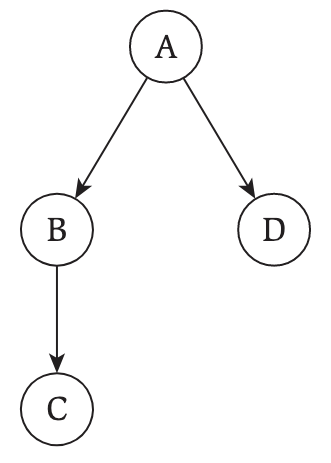
\includegraphics[width=0.15\textwidth]{q3.png}
    \caption{A hierarchy with four people. The fastest broadcast scheme is for A to call B in the first round. In the second round, A calls D and B calls C. If A were to call D first, then C could not learn the news until the third round.}
    \label{fig:q3}
\end{SCfigure}

\newpage

Give an efficient algorithm that determines the minimum number of rounds needed for everyone to be notified, and outputs a sequence of phone calls that achieves this minimum number of rounds by answering the following: 
\begin{parts}
\item Give a recursive algorithm. (The algorithm does not need to be efficient)
\begin{solutionbox}{\stretch {2}} \\
Let's represent the schedule as a list of lists 'A' that contains the calls done at round i in A[i]. \\
Input: An officer o with a list of subordinates [$s_{1},...,s_{n}$] where n is the number of subordinates\\
Output: (Number of rounds required for all the subordinates to get notified, schedule of the calls)\\
Algorithm: CallSchedule\\
if (n = 0) then:  //meaning the officer o has no subordinates\\
    return (0, [])\\
end-if\\
List = []  //initialize an empty list\\
for-each $s_{i}$ do:  //for each subordinate of officer o\\
    List.append(CallSchedule($s_{i}$))\\
end-for-each\\
Sort List by the first entry;\\
NumRounds = max(List[i][1] + i);\\
Schedule = schedule: at round 1, $s_{1}$; at round 2, $s_{2}$ and round 1 of $s_{1}$'s schedule, and so on;\\
return (N,S);
\end{solutionbox}

\item Give an efficient dynamic programming algorithm.
\begin{solutionbox}{\stretch 3} \vspace{1em} \\
Let A(v) denote the minimum number of rounds needed to contact all subordinates in the subtree rooted at v (ranking officer). Let $S_{v}[1,...,n]$ denote the list of direct subordinates i of v ordered by decreasing value of R(i). Then, the Bellman equation is given by:
\[ R(v) = max_{i = 1,..,n} (i + R(S_{v}[i]))\]
Then, the solution to the problem is R(ranking offer).
To get the schedule, we can think of $S_{v}$ as a tree. We can keep a stack of nodes such that its children are not exhausted. We initialize the stack with the top officer. At each round, we pop off all the nodes in the list. For each of the nodes v, we add the next children c of the nodes in $S_{v}$ not yet considered to the schedule at that round. And we add c to the stack. If there are still more children left for v, we add it back to the stack. We repeat this until the stack is empty.\\
Let m denote the number of nodes in the tree. There are m entires, and we sort each time taking O(m log m), so the runtime is O($m^2 log\ m$). The work we actually do to compute each $R_{v}$ is O($n_{v} log\ n_{v}$) if $n_{v}$ denotes the number of children of v. Since each node has a unique parent, the local work is $\sum_{v} O(n_{v} log\ n_{v})$ with $\sum_{v} n_{v} \approx m$. For any a,b > 0, we have a log a + b log b $\leq$ (a+b) log(a+b). So, the total work done is O(m log m ) for computing R. The backtracking step to check the correctness takes linear time because the number of times each node gets added to the stack is equal to the number of children it has. Meaning, each node adds its parent to the stack at most once, so it takes linear time with respect to m. Therefore, in total, the runtime is O(m log m).
\end{solutionbox}

\newpage

\item Prove that the algorithm in part (b) is correct.
\begin{solutionbox}{\stretch 2} \vspace{1em} \\
You can get the correctness of the above algorithm from the correctness of the Bellman equation, and we can prove this using strong induction.\\
Let's say we are considering the sequence of the calls for a node v. Given any sequence of calls by v, say ($u_{1},..,u_{n}$), the minimal possible rounds needed for the sequence is at least each of i + R($u_{i}$), since $u_{i}$ needs to make calls for its subordinates after it gets called by v at the ith round. Therefore, $R(v) = min_{(u_{1},..,u{n})} max_{i=1,..,n}(i + R(u_{i}))$.\\
Now, let's suppose U = ($u_{1},..,u_{n}$) is not sorted by the decreasing R values. That means there is some indices i < j such that $R(u_{i}) < R(u_{j}))$ and also $i + R(u_{i}) < j + R(u_{j})$. Let's consider a new sequence W = $(w_{1},..,w_{n})$ that is the same as U except we swap the $u_{i}$ and $u_{j}$. Then, $i + R(w_{i}) = i + R(u_{j}) < j + R(u_{j})$ and $j + R(w_{j}) = j + R(u_{i}) < j + R(u_{j})$. Therefore, removing an inversion in the sequence U does not increase the maximum value achieved. By the exchange argument, we can conclude that the minimal value is achieved when the sequence is sorted by the decreasing R value.
\end{solutionbox}
\end{parts}

\newpage

%%%%%%%%%

\question 
Consider the following problem: you are provided with a two dimensional matrix $M$ (dimensions, say, $m \times n$). 
Each entry of the matrix is either a \textbf{1} or a \textbf{0}. 
You are tasked with finding the total number of square sub-matrices of $M$ with all \textbf{1}s. 
Give an $O(mn)$ algorithm to arrive at this total count by answering the following:

\begin{parts}
  \item Give a recursive algorithm. (The algorithm does not need to be efficient)
  \begin{solutionbox}{\stretch 1}\vspace{1em}\\
    Algorithm: SquareSubMatrix\\
    Input: M = m x n binary matrix\\
    Output: the number of square submatrices of M with all 1\\
    if m = 0 then: //base case \\
        return 0;\\
    end-if\\
    N = SquareSubMatrix(M[2,..,m][1,..,n]);\\
    for-each i $\in$ [1,..,n] do:\\
        k = number of square submatrices with all 1 having M[1,i] as its upper left corner;\\
        N = N + k;\\
    end-for-each\\
    return N;\\
  \end{solutionbox}
  
  \item Give an efficient dynamic programming algorithm.
  \begin{solutionbox}{\stretch 1} \vspace{1em} \\
       Let A(i,j) denote the side length of the biggest square submatrix with 1s and with bottom-right corner at M[i][j]. Note that this number A(i,j) also counts the number of square submatrix with 1s with bottom-right corner at M[i][j].\\
       \begin{equation*}
        A(i,j) =
        \begin{cases}
            M[i][j] & \text{ if i = 0 or j = 0}\\ 
            0 & \text{ if M[i][j] = 0}\\
            min(A(i-1,j), A(i,j-1), A(i-1, j-1)) + 1 & \text{if M[i][j] = 1}
        \end{cases}
    \end{equation*}
    We can solve this recurrence relation directly using a recursive algorithm. The solution is then $\sum_{i,j} A(i,j)$.\\
    We are basically filling up a table of size m x n with constant amount of work for each entry. Therefore, the runtime is O(mn).
  \end{solutionbox}
 \newpage 
  \item Prove that the algorithm in part (b) is correct.
  \begin{solutionbox}{\stretch 2} \vspace{1em} \\
  The recurrence relation given above is correct because the largest square 1 matrix with M[i][j] at the bottom-right corner is constrained by the largest such matrices at M[i-1][j], M[i][j-1], and M[i-1][j-1]. We can think of this also as: suppose length l square is the largest 1 square matrix we can fit with bottom-right corner at M[i][j]. This square also includes three length (l-1) 1 squares with bottom-right corner at M[i-1][j], M[i][j-1], and M[i-1][j-1]. Therefore, A(i,j) $\leq$ A(i-1,j) + 1, A(i,j) $\leq$ A(i,j-1) + 1, and A(i,j) $\leq$ A(i-1,j-1) + 1, so A(i,j) $\leq$ min(A(i-1,j),A(i,j-1),A(i-1,j-1)) + 1. For the other direction, we can see one of the above three inequalities must be equal, because if not, then we would be able to fit length l squares at each of those three corners, giving us a length l + 1 square fitting at the corner M[i][j]. That is equivalent to taking the minimum of the three A values. 
  \end{solutionbox}

  \item Furthermore, how would you count the total number of square sub-matrices of $M$ with all \textbf{0}s?
  \begin{solutionbox}{\stretch 1} \vspace{1em}\\ 
  All we need to do is convert M to M'. M' has the opposite entries of M and we can use our algorithm on M'.
  \end{solutionbox}
  \end{parts}
\newpage

%%%%%%%%


\question \textit{Kleinberg, Jon. Algorithm Design (p. 329, q. 19).} 

String $x'$ is a \emph{repetition} of $x$ if it is a prefix of $x^k$ ($k$ copies of $x$ concatenated
together) for some integer $k$. So $x' = 10110110110$ is a repetition of $x = 101$.
We say that a string $s$ is an \textit{interleaving} of $x$ and $y$ if its symbols can be partitioned into two (not necessarily contiguous) subsequences $x'$ and $y'$, so that $x'$ is a repetition of $x$ and $y'$ is a repetition of $y$. 
For example, if $x = 101$ and $y = 00$,
then $s = 100010010$ is an interleaving of $x$ and $y$, since characters $1,2,5,8,9$ form $10110$—a repetition of $x$—and the remaining characters $3,4,6,7$ form
$0000$—a repetition of $y$.

Give an efficient algorithm that takes strings $s$, $x$, and $y$ and decides if $s$ is an interleaving of $x$ and $y$ by answering the following:

\begin{parts}
  \item Give a recursive algorithm. (The algorithm does not need to be efficient)
  \begin{solutionbox}{\stretch 2} \vspace{1em} \\
  Let's assume that we have long enough X = $x^{k}$ and Y = $y^{k}$ for some big enough k.\\
  Algorithm: InterLeaving\\
  Input: Strings s, X, and Y\\
  Output: Whether s is an interleaving of X and Y or not\\
  //base case\\
  if length of s = 0 then:\\
    return True;\\
  end-if\\
  if s[0] $\neq$ X[0] $\textasciicircum$ s[0] $\neq$ Y[0] then:\\
    return False:\\
  end-if\\
  $b_{X}, b_{Y}$ = False;\\
  if s[0] = X[0] then:\\
    $b_{X}$ = InterLeaving(s, X[2,..], Y);\\
  end-if\\
  if s[0] = Y[0] then:\\
    $b_{Y}$ = InterLeaving(s, X, Y[2,..]);\\
  end-if\\
  return $b_{X} \vee b_{Y}$;
  \end{solutionbox}
  
  \item Give an efficient dynamic programming algorithm.
  \begin{solutionbox}{\stretch 1} \vspace{1em} \\
  Let x' and y' be the infinite repetition of x and y respectively. Let A(i,j) denote whether the substring $a_{1}, a_{2},..,a_{i+j}$ is an interleaving if $x_{1}^{'},..,x_{i}^{'}$ and $y_{1}^{'},..,y_{j}^{'}$.
  \[ A(i,j) = [A(i-1, j) \textasciicircum (s_{i+j} == x_{i}^{'})] \vee [A(i, j-1) \textasciicircum (s_{i+j} == y_{j}^{'})]\]
  The base case for this is A(0,0) = 1, A(i,0) = ($a_{i} == x_{i}^{'}$) and A(0,j) = ($a_{i} == y_{j}^{'}$). The output will be true if there is some i + j = l with A(i,j) being true. We only need finite initial segment of x' and y'. Also, $x_{i}^{'} = x_{i} \mod{l}$ where l is the length of x, so it can be computed in constant time. Therefore, it takes $O(n^2)$ time since i and j are in range 0 to n where n is the length of a. 
  \end{solutionbox}
 
  \newpage
  \item Prove that the algorithm in part (b) is correct.
  \begin{solutionbox}{\stretch 1} \vspace{1em} \\
  The best cases for this algorithm come out to be true.\\
  Let's assume that A(i, j-1) and A(i-1,j) return the correct result. The string $a_{1},..,a_{i+j}$ can be interleaved with $x_{1}^{'},..,x_{i}^{'}$ and $y_{1}^{'},..,y_{j}^{'}$ if and only if the last character of the string, $a_{i+j}$ matches with one of the $x_{i}^{'}$ and $y_{j}^{'}$. The recurrence relation expresses this statement. Also, we need to check for all the possible repetitions of x and y.
  \end{solutionbox}
  \end{parts}


%%%%%%%%%

\question \textit{Kleinberg, Jon. Algorithm Design (p. 330, q. 22).} 

To assess how “well-connected” two nodes in a directed graph are, one can not only look at the length of the shortest path between them, but can also count the number of shortest paths. 

This turns out to be a problem that can be solved efficiently, subject to some restrictions on the edge costs. Suppose we are given a directed graph $G = (V, E)$, with costs on the edges; the costs may be positive or negative, but every cycle in the graph has strictly positive cost. We are also given two nodes $v, w\in V$. 

Give an efficient algorithm that computes the number of shortest $v-w$ paths in $G$. (The algorithm should not list all the paths; just the number suffices.) 

  \begin{solutionbox}{\stretch 2} \vspace{1em} \\
  We keep track of two 2D matrices A and B such that A[n][i] the cost of the shortest path from i to w of length exactly n, and B[n][i] is the number of such paths. We initialize A[1][i] = $a_{iw}$ and B[1][i] = 1 if there is an edge (i,w) $\in$ E and A[1][i] = $\infty$ and B[1][i] = 0 otherwise.\\
  We update the entries of A and B as follows:\\
  \[ A[n][i] = min_{j \in V} (a_{ij} + A[n-1][j])\]
  and
  \[ B[n][i]= \sum_{j} B[n-1][j] \text{\ \ \ \ for $j \in V$ with $a_{ij} A[n-1][j] = A[n][i]$}\]
  To find the solution, we first compute the cost of the shortest path from v to w, which is a = $min_{1 \leq n \leq \mod{V} -1} A[n][v]$. Then, for each j with A[j][v] = a, we return b = $\sum_{j} = B[j][v]$.\\
  To show correctness, we fix the n. Suppose a is the cost of the shortest path from i to w of length n. And suppose b is the number of such paths. Then, if $p_{1}, p_{2},..,p_{m}$ are those paths, the cost of each one of them are a and they all have length n. We can partition them disjointly by the first vertex visited after i. Suppose WLOG, that $p_{1},..,p_{k}$ start with the edge (i,j).\\
  If $p_{1}^{'},..,p_{k}^{'}$ denote the paths obtained by removing the first edge, then they must be the shortest path from j to w of length n-1. Then, by an inductive argument, k = B[n-1][j] and the cost of each of the must be A[n-1][j] = $a - a_{ij}$. Also, since there is no negative cycle, all shortest paths must have length less than n, so the algorithm counts them all.
  \end{solutionbox}

\newpage

%%%%%%%%%

\question The following is an instance of the Knapsack Problem. 
Before implementing the algorithm in code, run through the algorithm by hand on this instance. 
To answer this question, generate the table, indicate the maximum value, and recreate the subset of items.

\begin{center}
\begin{tabular}{ |c|c|c| } 
 \hline
 item & weight & value \\ 
\hline
\hline
 1 & 4 & 5 \\ 
\hline
 2 & 3 & 3 \\ 
\hline
 3 & 1 & 12 \\ 
\hline
 4 & 2 & 4 \\ 
 \hline
\end{tabular}

Capacity: 6
\end{center}
  \begin{solutionbox}{\stretch 1} \vspace{1em} 
    \begin{center}
    \begin{tabular}{ |c|c|c|c|c|c|c|c| } 
    \hline
    4 & 0 & 12 & 12 & 16 & 16 & 17 & 19 \\ 
    \hline
    3 & 0 & 12 & 12 & 12 & 15 & 17 & 17 \\ 
    \hline
    2 & 0 & 0 & 0 & 3 & 5 & 5 & 5 \\ 
    \hline
    1 & 0 & 0 & 0 & 0 & 5 & 5 & 5 \\  
    \hline
    0 & 0 & 0 & 0 & 0 & 0 & 0 & 0 \\ 
    \hline
     & 0 & 1 & 2 & 3 & 4 & 5 & 6 \\ 
    \hline
\end{tabular}
\end{center}

Maximum value: 19\\
Items used: 2, 3, 4\\
  \end{solutionbox}


\newpage

\question \textbf{Coding Question: Knapsack}

Implement the algorithm for the Knapsack Problem in either C, C++, C\#, Java, Python, or Rust. Be efficient and implement it in $O(nW)$ time, where $n$ is the number of items and $W$ is the capacity.

The input will start with an positive integer, giving the number of instances that follow. For each instance, there will two positive integers, representing the number of items and the capacity, followed by a list describing the items.
For each item, there will be two nonnegative integers, representing the weight and value, respectively.

A sample input is the following:

\begin{verbatim}
2
1 3
4 100
3 4
1 2
3 3
2 4
\end{verbatim}
The sample input has two instances. The first instance has one item and a capacity of 3. The item has weight 4 and value 100. 
The second instance has three items and a capacity of 4.

For each instance, your program should output the maximum possible value.
The correct output to the sample input would be:

\begin{verbatim}
0 
6
\end{verbatim}


\end{questions}

\end{document}
